\section{Beyond the Standard Model}
\label{section:BSM}

Beyond the \acrshort{SMlabel} (\acrshort{BSMlabel}) theories aim to extend or replace the \acrshort{SMlabel} by addressing its limitations and shortcomings. Several theories have been proposed to address some of the questions mentioned in the previous section, and among them are the extended Higgs sectors and flavon models. Overall, \acrshort{BSMlabel} theories provide a rich landscape of new physics, and their predictions can be tested by current and future experiments.

\subsection{Two Higgs Doublet Model}

The Two Higgs Doublet Model (2HDM) extends the \acrshort{SMlabel} by adding a second Higgs doublet. With two scalar Higgs doublets, the electroweak symmetry can be broken differently and the type of model can be defined depending on which fermions couple to each doublet. One of the most studied is the Type-II 2HDM, in which up-type quarks couple to one doublet while the down-type quarks and charged leptons couple to the other,

\begin{equation}
    \Phi_1\equiv H_u = 
    \begin{pmatrix} H^+_u \\ H^0_u \end{pmatrix} =
    \frac{1}{\sqrt{2}}
    \begin{pmatrix} 0 \\ v_u \end{pmatrix},
    \qquad
    \Phi_2\equiv H_d = 
    \begin{pmatrix} H^-_d \\ H^0_d \end{pmatrix} =
    \frac{1}{\sqrt{2}}
    \begin{pmatrix} 0 \\ v_d \end{pmatrix}
\end{equation}

with $v_u$ and $v_d$ being the \acrshort{VEV} of each doublet field. This scalar sector has eight initial degrees of freedom, four more than in the \acrshort{SMlabel}, yielding a total of five physical scalars instead of just the \acrshort{SMlabel} Higgs. The predicted particles are two neutral CP-even scalars $h$ and $H$ ($m_h < m_H$), one CP-odd pseudo-scalar $A$ and two charged Higgs bosons $H^\pm$. This type of models have six free parameters: $m_h$, $m_H$, $m_A$, $m_{H^\pm}$, $\tan\beta$ and $\alpha$. The last two are the ratio of the two \acrshort{VEV}, $\tan\beta=\frac{v_u}{v_d}$, and a mixing angle $\alpha$ that diagonalises the mass matrix of the CP-even states. 

\subsection{Supersymmetry}

Supersymmetry (SUSY) is a popular theoretical extension of the \acrshort{SMlabel} that solves many issues of the \acrshort{SMlabel} like the hierarchy problem or proposing a DM particle. It is a framework of theories that introduces a symmetry between the fermion and boson sectors (supersymmetry), predicting a superpartner particle with different spin for each \acrshort{SMlabel} particle. No new particles or other experimental evidence have been found so far; however, there are many SUSY models with different assumptions and parameters that still remain consistent with the current experimental data and could potentially be discovered.\\

The simplest realization of SUSY is the Minimal Supersymmetric~\acrshort{SMlabel} (MSSM), one of the models best studied and motivated. The model introduces the minimal amount of additional degrees of freedom with respect to the \acrshort{SMlabel}, with new particles and no new interactions. Every \acrshort{SMlabel} particle has an associated superpartner with different spin: the SUSY particles related to the \acrshort{SMlabel} gauge bosons are known as gauginos, the squarks are related to quarks, sleptons to leptons and Higgsinos to the Higgs bosons. The MSSM has an additional Higgs doublet to prevent anomalies from the Higgsino, therefore it is a 2HDM theory and predicts five physical scalars, as mentioned before.\\

In addition, a new quantum number is introduced, the $R$-parity,

\begin{equation}
    R=(-1)^{3(B-L)+2S}
\end{equation}

where $B$ is the baryon number, $L$ is the lepton number, and $S$ is the spin. The parity has a value of $+1$ for \acrshort{SMlabel} particles and -1 for the SUSY particles. The $R$-parity is conserved in the MSSM and, as one of the consequences, the lightest SUSY particle (LSP) is stable and has a negligible coupling with the \acrshort{SMlabel} particles making it a candidate for DM.\\

Since the discovery of the Higgs boson, it is usual to interpret either of the CP-even neutral scalars ($h$ or $H$) of the theory to be the SM Higgs. One method to do this is by working in the decoupling limit, where all the SUSY particles and non-standard Higgs bosons are assumed to be much heavier than the \acrshort{EW} scale, making the $h$ scalar behave just like the SM Higgs boson. Another method involves comparing the \acrshort{SMlabel} Higgs couplings to the different \acrshort{SMlabel} particles. The hMSSM model~\cite{arxiv.1502.05653} is a simplified version of the MSSM, and the couplings of the new Higgs particles to the \acrshort{SMlabel} can be easily written and compared to the \acrshort{SMlabel} Higgs couplings,


\begin{align}
    \begin{split}
    g_{H_\text{SM}VV}\quad &\rightarrow\quad H_\text{SM} = H \cos(\beta-\alpha)+h\sin(\beta-\alpha)\\
    g_{H_\text{SM}u\bar{u}}\quad &\rightarrow\quad H_\text{SM} = H \frac{\sin\alpha}{\sin\beta}+h\frac{\cos\alpha}{\sin\beta}\\
    g_{H_\text{SM}d\bar{d}}\quad &\rightarrow\quad H_\text{SM} = H \frac{\cos\alpha}{\cos\beta}-h\frac{\sin\alpha}{\cos\beta}
\end{split}
\end{align}

with $V$ being the massive gauge bosons. Taking the so-called alignment limit, $\cos(\beta-\alpha)\to 0$, the $h$ behaves like the \acrshort{SMlabel} Higgs, while $H$ becomes gauge-phobic. The couplings to gauge bosons are particularly important, as they arise from the gauge invariance and do not depend on the particular MSSM model.\\

In this thesis, hMSSM model predictions are used as it is a very simplified model focused on the Higgs sector, making it easy to study. This is primarily due to the presence of only two free parameters in the Higgs sector: $M_A$ and $\tan\beta$. Apart from the alignment limit, the model has different assumptions that lead to the $h$ mass set to the \acrshort{SMlabel} Higgs mass, the Higgs couplings to depend only on the angles, and with the phenomenology to not depend on the usual SUSY parameters, like the SUSY scale ($M_S$). However, even if the $\tan\beta$ and $M_{A}$ can have a wide range of possible values, the implication of reaching very low values of $\tan\beta$ ($<<1$) is to consider a large $M_S$ scale or other fine-tuned scenarios. On the other hand, high values of $\tan\beta$ ($>>50$) push the $M_S$ towards the \acrshort{EW} scale, which has been ruled out for many years. Although it is convenient to obtain predictions from the hMSSM model, the underlying SUSY parameters have important phenomenological implications and their elusion in the model is not always appropriate to define benchmark scenarios. \\

Five additional benchmark models~\cite{Bagnaschi_2019} designed for MSSM Higgs searches are contemplated in this thesis. In contrast to the hMSSM, they are updated with current \acrshort{LHClabel} results and fix the different underlying SUSY parameters. The $\text{M}^{125}_\text{h}$, $\text{M}^{125}_\text{h}$($\tilde{\chi}$), $\text{M}^{125}_{\text{h}_1}$($\tilde{\tau}$), $\text{M}^{125}_\text{h}$(alignment) and $\text{M}^{125}_\text{h}$(CPV) have two free parameters, $\tan\beta$ and $M_A$, and are designed to accommodate one of the CP-even Higgs bosons close to 125 GeV, while preserving the key features of the MSSM Higgs sector. The $\text{M}^{125}_\text{h}$ model, also known as the 'vanilla' scenario, focuses on the decoupling limit where the heavy Higgs states are decoupled from the light ones, providing a Higgs boson similar to the \acrshort{SMlabel}. The $\text{M}^{125}_\text{h}$($\tilde{\chi}$) model incorporates light neutralinos as the lightest SUSY particles (LSPs), accounting for potential dark matter candidates in the MSSM. The $\text{M}^{125}_{\text{h}1}$($\tilde{\tau}$) scenario explores the possibility of enhanced third-generation couplings, particularly through the involvement of stau (the SUSY partner of the tau lepton) co-annihilation processes. This model helps to probe the impact of the SUSY sector on the Higgs sector. The $\text{M}^{125}_\text{h}$(alignment) scenario focuses on the alignment limit. Lastly, the $\text{M}^{125}_\text{h}$(CPV) scenario investigates the explicit CP violation in the Higgs sector, which can result from complex phases in the MSSM parameters. This can lead to a mixing of the CP-even and CP-odd Higgs states, affecting their masses and couplings.

\subsection{Dark Matter and the 2HDM+a model}

The 2HDM+a model~\cite{Bauer_2017,10.48550/arxiv.1810.09420} is an extension of the 2HDM that incorporates a simplified Dark Matter~(DM) sector, consisting of a single fermionic DM particle ($\chi$) and a pseudo-scalar mediator ($a$) on top of the two complex Higgs doublets in the Higgs sector. In this particular model, the interactions between the \acrshort{SMlabel} and DM sectors are mediated by the pseudo-scalar $a$, although other models consider axial-vectors or scalars~\cite{Abercrombie_2020,10.48550/arxiv.1603.04156,10.48550/arxiv.1703.05703}. The choice of a pseudo-scalar is motivated by the potential sensitivity in collider searches, as direct detection of pseudo-scalars is suppressed~\cite{Abe_2019} and a dedicated search will not provide strong constraints.\\

The phenomenology of the model includes the five Higgs bosons from the 2HDM sector: a light CP even boson $h$, a heavy CP-even boson $H$, a CP-odd boson $A$ and the charged bosons $H^\pm$. As in the previous models, the Type-II structure is considered together with the alignment limit~\cite{Gunion_2003}, to identify the $h$ state with the \acrshort{SMlabel} Higgs boson. The mediator $a$ couples the \acrshort{SMlabel} fermions with the Dirac DM particle $\chi$. In addition, $a$ couples to \acrshort{SMlabel} fermions proportionally to the Yukawa couplings and mixes with $A$ through a mixing angle $\theta$.

A total of 14 parameters are required to fully determine the model: the masses of the five 2HDM Higgs bosons; the mass of the mediator $a$; the mass of the DM particle $\chi$; the coupling between $a$ and $\chi$, $g_\chi$; the \acrshort{EW} \acrshort{VEV}, $v$; the ratio of the 2HDM \acrshort{VEV}s, $\tan\beta$; the mixing angles of the CP-even and CP-odd states, $\alpha$ and $\theta$, respectively; and three quartic couplings between the scalar doublets and the mediator.\\

This model predicts a wide variety of signatures and \acrshort{ATLASlabel} has summary results that consist in various dark matter searches using 139~fb$^{-1}$ data~\cite{Hpluscomb}. The most prominent signatures, the production of DM in association with a Higgs boson $\MET+h(\bbar)$~\cite{2108.13391} and with a $Z$ boson $\MET+Z(\ell^+\ell^-)$ are used in a combined likelihood fit for the statistical combination. Further signatures are related to DM production in association with a top quark and a W boson (\MET+$Wt$), visible decays of the additional heavy Higgs bosons, and invisible decays of the SM Higgs boson to DM.\\

\subsection{The flavon in top-quark FCNC decays}

Several extensions of the \acrshort{SMlabel} predict enhanced top-quark FCNC decays. Among these extensions are the quark-singlet model~\cite{PhysRevD.67.035003}, the 2HDM with or without flavor-conservation~\cite{B_jar_2001,GUASCH19993,Cao_2007}, SUSY with R-parity violation~\cite{Eilam_2001}, and composite Higgs models with partial compositeness~\cite{Azatov2014}. These theories introduce FCNC contributions at tree level and can enhance the top-quark FCNC decay branching fractions by orders of magnitude. In the context of 2HDM, the presence of two Higgs doublets can give rise to tree-level FCNCs in the Higgs sector if the doublets couple to both up- and down-type quarks (2HDM Type-III). Similarly, SUSY models with R-parity violation can introduce couplings between quarks and squarks resulting in FCNC processes mediated by squarks.\\

Other extensions of the \acrshort{SMlabel} predict the existence of new particles, either a neutral scalar, a pseudoscalar or an axion-like particle. In these models, the new particle couples to the top-quark and introduces FCNC couplings. One specific model that predicts enhanced top-quark FCNC decays is the Froggatt-Nielsen mechanism~\cite{FROGGATT1979277,Banerjee2018}. In a simple expression of the model~\cite{Bauer_2016}, the SM is extended by introducing a new Abelian flavour symmetry $U(1)_F$ and a scalar field $X$, known as the flavon, which carries flavour charge. The flavon field acquires a \acrshort{VEV} when the $U(1)_F$ symmetry is spontaneously broken. When breaking the symmetry, the mass hierarchy of the fermions is generated as the Yukawa couplings of the flavon depend on the flavour charges of the quarks.\\

The flavon can be produced in top-quark FCNC decays such as the $t\to uX$ and $t\to cX$ processes. Since the flavon has larger couplings to third-generation quarks, the $t\to cX$ process is more relevant, with the dominant decay mode $X\to b\bar{b}$ for masses below 200~GeV. Figure~\ref{BSM:flavon} shows the top-quark branching ratios involving the flavon, $t\to cX$ and $t\to uX$, and the flavon branching rations for decays to quarks.

\begin{figure}[htbp]
    \RawFloats
    \begin{center}
        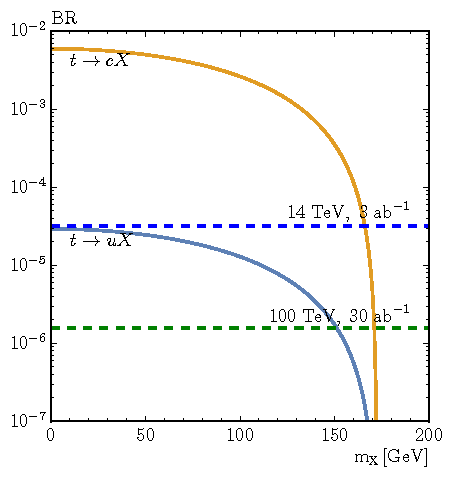
\includegraphics[width=0.49\textwidth]{SM/flavonproduction.pdf}
        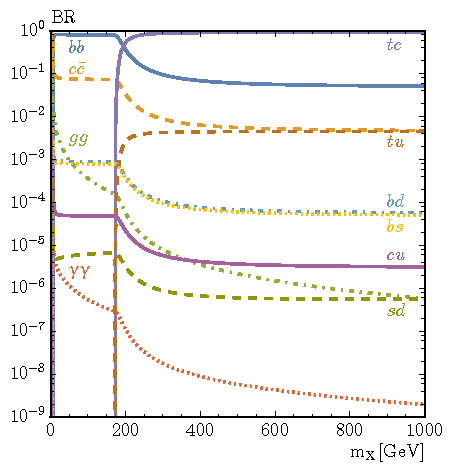
\includegraphics[width=0.49\textwidth]{SM/flavondecay.pdf}
        \caption{
        Branching fraction of the top-quark into a flavon and either $u$- or $c$-quarks (left) and flavon branching ratios for decays to quarks (right) as a function of the flavon mass, $m_X$~\cite{Bauer_2016}. The top-quark branching fraction are computed assuming a fixed \acrshort{VEV} 500~GeV.
    }
    \label{BSM:flavon}
    \end{center}
\end{figure}


%https://arxiv.org/pdf/1502.05653.pdf hmmsm
%https://arxiv.org/pdf/1808.07542.pdf mh125


% Decide what to explain of 2HDMs, hmmsm different to mh125 i have the referneces

% Charged Higgs phenomenlogy (production and decay)

% As discussed in Section 1.2.3 FCNC measurements, FCNC processes are heavily suppressed in the SM, yielding BR unreachable by the current accelerators. Nevertheless, it makes FCNC searches a great candidate for BSM as any proof of FCNC at the reachable sensitivity would point to a theory that introduces this type of interactions or slightly modifies the GIM mechanism.

% Flavon -> types of mechanisms -> U(1) (check paper and internal note)
% Flavon, prediction and decay aswell?
% assuming f / lambda sm to be cabibo angle 0.23???


% ---
% CONF %https://cds.cern.ch/record/2777863/files/ATLAS-CONF-2021-036.pdf
% The ATLAS experiment [6] at the Large Hadron Collider (LHC) [7] is a general-purpose detector that allows
% for a wide range of DM searches. In the following, the focus will be entirely on the hypothesis that DM is a
% weakly interacting massive particle (WIMP) [8] and, more specifically, a Dirac fermion. WIMPs could in
% principle interact with the SM sector in different ways. A particular strength of collider searches lies in the
% fact that the high-energy collisions of SM particles could not only produce DM directly under controlled
% experimental conditions but also provide access to particles mediating the interactions between DM and
% the SM sector. A mediator produced in a collision could decay to DM particles, which themselves could
% not be detected and would lead to missing transverse momentum (with magnitude \MET). Alternatively, a
% mediator could decay back into SM particles, from which its properties could be reconstructed.
% Dark matter searches at the LHC explore both avenues in the quest to solve the puzzle of DM. Invisible
% mediator decays can be detected only if the mediator is produced in association with another particle,
% for example from initial-state radiation that results in a hadronic jet, leading to a characteristic \MET+jet
% signature [9, 10]. Visible mediator decays allow for the reconstruction of the mediator particle from
% its decay products, for example in the context of resonance searches, if the mediator is produced in the
% s-channel [11-15].

% The above-mentioned searches are traditionally interpreted in the context of so-called simplified models of
% DM, which rely on a minimal set of new particles and interactions. The most commonly used among these
% simplified models postulate the existence of a single fermionic DM particle and a single mediator, which,
% depending on the model, could be a vector, axial-vector, scalar, or pseudo-scalar particle [16-18]. The
% models are characterised by a minimal set of free parameters, namely the masses of the DM and mediator
% particles and the couplings of the mediator to the SM and dark sectors.

% In this note, a more complete benchmark model is used. It provides an ultra-violet complete and
% renormalisable framework for the interpretation of DM searches. It is built upon the assumption that the
% SM Higgs boson is part of an extended Higgs sector with two complex Higgs doublets. This is a key
% assumption in many theories extending the SM, such as supersymmetry [19]. The interaction between the
% SM sector and DM in this model is mediated by a pseudo-scalar particle a. pseudo-scalar mediators are not
% strongly constrained by direct-detection experiments because the tree-level amplitude for the DM-nucleon
% elastic scattering is suppressed by the momentum transfer in the non-relativistic limit [20]. This renders
% collider searches for these processes particularly useful.

% The model, referred to as Two Higgs Doublet Model (2HDM) + pseudo-scalar mediator (a), 2HDM+a, is
% the simplest and currently only gauge-invariant and UV-complete extension of the simplified model with a
% pseudo-scalar mediator, and has been first introduced in Ref. [21]. The model is adopted as a common LHC
% benchmark model by the LHC Dark Matter Working Group [22], which is a joint forum of theory groups
% and the ATLAS, CMS, and LHCb collaborations. This model, unlike the simplified models described above,
% predicts a wide variety of detector signatures. Among the most prominent signatures in the parameter space
% explored in this note are the production of DM in association with a Higgs boson (\MET+h signatures) or
% with a Z boson (\MET+Z signatures). Further signatures are related to DM production in association with
% a top quark and a W boson (\MET+Wt), visible decays of the additional heavy Higgs bosons, and invisible
% decays of the SM Higgs boson to DM.
% A summary paper including constraints on the 2HDM+a benchmark based on a variety of dark matter
% searches using 36 fb$^{-1}$ data of sqrts = 13 TeV proton-proton collisions has been previously published by the
% ATLAS Collaboration [23]. Constraints on the model have also been derived by the CMS Collaboration
% using the results from searches in the \MET+ h(\bbar) [24] and \MET.
% -------------------------